\chapter{Validation, limites et perspectives}
\section{Méthode de validation}
La validation proposée repose sur des scénarios métier plutôt que sur un déploiement industriel. Chaque scénario doit être relié à un problème, à un ensemble de use cases, à un diagramme UML et à un composant applicatif.

\begin{figure}[H]
\centering
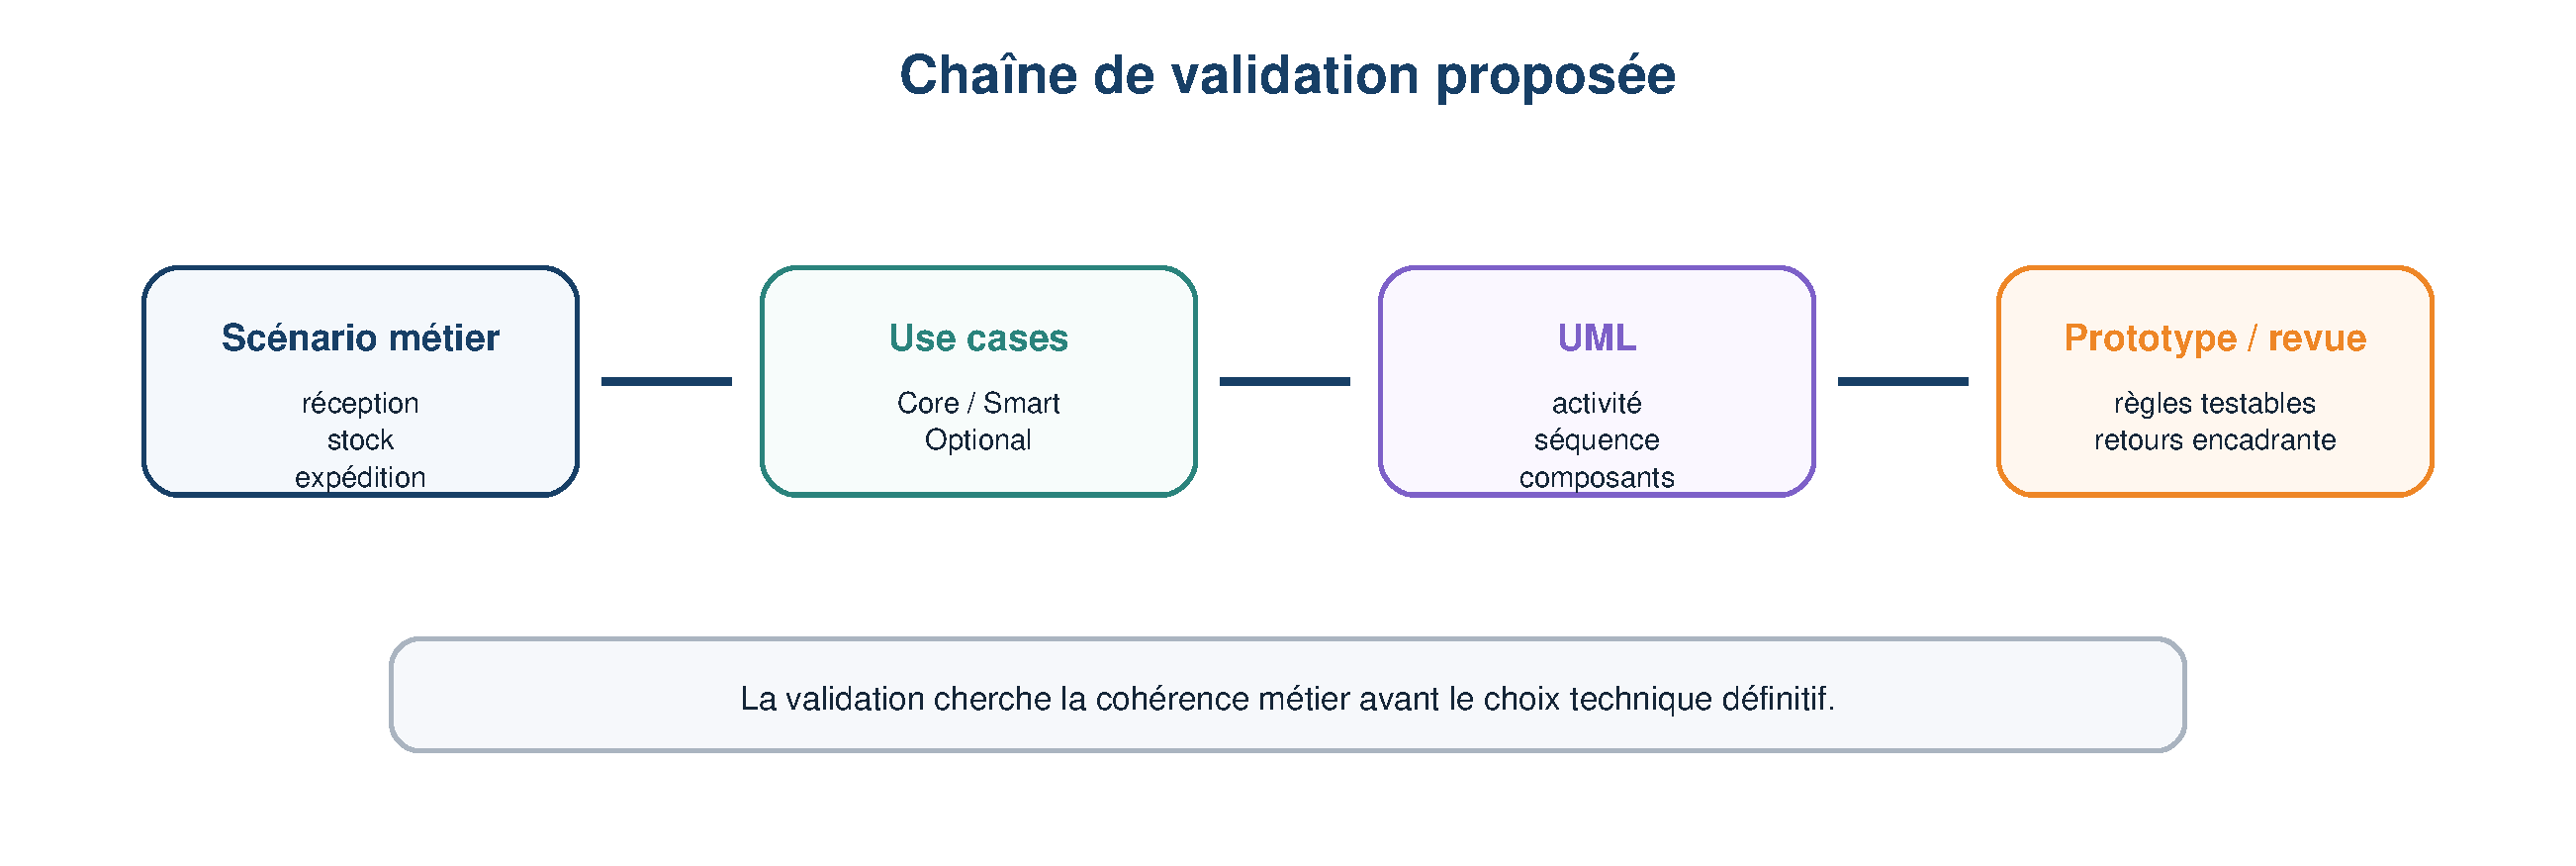
\includegraphics[width=0.88\linewidth]{figures/chapitre7/chaine_validation.pdf}
\caption{Chaîne de validation proposée pour l'architecture Smart WMS.}
\label{fig:validation}
\end{figure}

\section{Limites}
Le benchmark reste limité aux informations disponibles et ne remplace pas une étude détaillée de licences, coûts, performances ou contraintes réglementaires. La modélisation UML n'a pas encore été validée sur un entrepôt réel. Les capacités IA restent conceptuelles ou démontrées par une maquette contrôlée, avec données synthétiques.

\section{Perspectives}
Les perspectives naturelles sont la simulation de scénarios réels, la collecte de jeux de données entrepôt, la création d'un dashboard de supervision, l'intégration d'un IoT gateway, l'évaluation de modèles de prévision, puis la connexion progressive avec ERP, WCS/WES ou BMS/EMS. Une attention particulière devra être portée à la qualité des données, à la sécurité, à la supervision humaine et à la traçabilité des recommandations.
